\begin{frame}{The Normal Distribution}
    We start our review with the \textbf{normal distribution}. This is one of the most common distributions you will see in practice.
    
    \begin{center}
        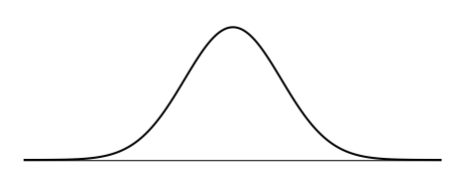
\includegraphics[scale=0.5]{images/normalcurve.png}
    \end{center}
\end{frame}

\begin{frame}{The Normal Distribution Model}
    \begin{itemize}
        \item The symmetric, unimodal, bell-shaped curve of the normal distribution can vary based on:
        \begin{itemize}
            \item Mean
            \item Standard deviation
        \end{itemize}
        \item These adjustable details are called \textbf{model parameters}.
    \end{itemize}
\end{frame}

\begin{frame}{Normal Distribution Notation}
    For a normal distribution with mean $\mu$ and standard deviation $\sigma$, we write
    \[
        N(\mu, \sigma)
    \]
    For a variable $X$ with a normal distribution, we may write
    \[
        X \sim N(\mu, \sigma).
    \]
    where "$\sim$" denotes "is distributed".
\end{frame}

\begin{frame}{Normal Distribution Notation}
    For a normal distribution with mean $19$ and standard deviation $4$, we write
    \[
        N(\mu=19, \sigma=4)
    \]
    \begin{itemize}
        \item The mean and standard deviation describe a normal distribution fully and exactly. 
        \item This is what we mean by a distribution's \textbf{parameters}.
    \end{itemize}
\end{frame}

\begin{frame}{Standard Normal Distribution}
    The \textbf{standard normal distribution} is a normal distribution with mean $\mu=0$ and standard deviation $\sigma=1$.
    \[
        N(\mu=0, \sigma=1)
    \]
\end{frame}

\begin{frame}{Standardizing with Z-Scores}
    We often want to put data onto a standardized scale, which can make comparisons more reasonable.
\end{frame}

\begin{frame}{Standardizing with Z-Scores}
    We compute the Z-score for an observation $x$ that follows a distribution with mean $\mu$ and standard deviation $\sigma$ using
    \[
        z = \frac{x-\mu}{\sigma}
    \]
\end{frame}

\begin{frame}{Example}
    Let $X$ represent a random variable from $N (\mu = 3, \sigma = 2)$
    \[
        X \sim N (\mu = 3, \sigma = 2)
    \]
    and suppose we observe $x = 5.19$.
    \begin{enumerate}
        \item Find the Z-score of x.
        \item Use the Z-score to determine how many standard deviations above or below the mean x falls.
    \end{enumerate}
\end{frame}

\begin{frame}{Example: Brushtail Possums}
    \begin{center}
        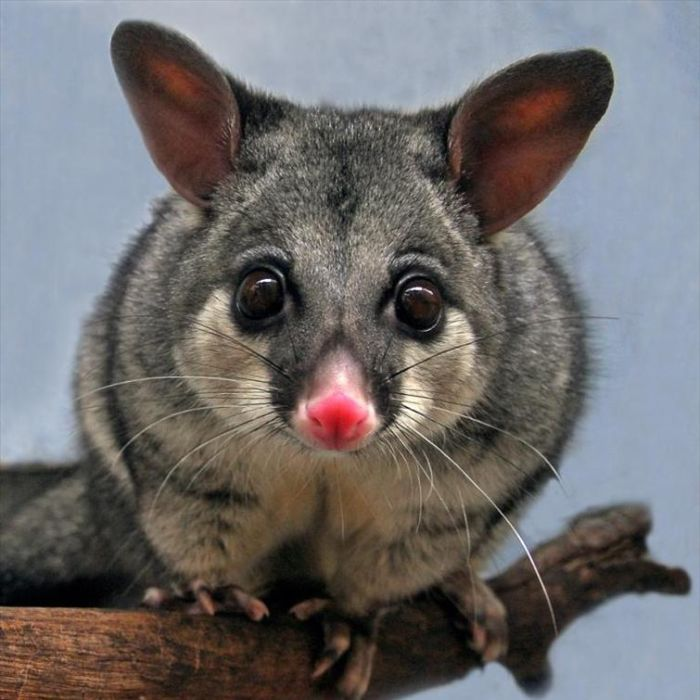
\includegraphics[scale=0.2]{images/possum.jpg}
    \end{center}
    Head lengths of brushtail possums follow a normal distribution with mean 92.6 mm and standard deviation 3.6 mm. 
    
    \vspace{12pt}Compute the Z-score for a possum with head length 85.8 mm.
\end{frame}

\begin{frame}{Finding Tail Areas}
    There are several techniques for finding tail areas:
    \begin{enumerate}
        \item Integrate.
        \item Use a graphing calculator.
        \item Use a probability table.
        \item Use a statistical software.
    \end{enumerate}
\end{frame}

\begin{frame}{Finding Tail Areas}
    \begin{itemize}
        \item For quizzes and exams, you will be provided with information from \texttt{R}. 
        \item I will do the work in \texttt{R}, but you may need to use a Z-score to pick the correct tail probability from a list.
    \end{itemize}
    For example
    \begin{center}
        \begin{tabular}{l l}
            \hline
            Z-score & Lower Tail Area \\
            \hline
            1 & 0.8413 \\
            1.5 & 0.9332 \\
            \hline
        \end{tabular}
    \end{center}
\end{frame}

\begin{frame}{Example: Normal Probability}
    Cumulative SAT scores are well-approximated by a normal model, $N (\mu = 1100, \sigma = 200)$.
    
    \vspace{12pt}Shannon is a randomly selected SAT taker, and nothing is known about her SAT aptitude. What is the probability Shannon scores at least 1190 on her SATs?
\end{frame}

\begin{frame}{Finding Areas to the Right}
    \begin{itemize}
        \item Software programs usually return the area to the left (left tail) when given a Z-score.
        \item To get the area to the right
        \begin{enumerate}
            \item Find the area to the left.
            \item Subtract this area from one.
        \end{enumerate}
    \end{itemize}
\end{frame}

\begin{frame}{Example}
    Edward earned a 1030 on his SAT. What is his percentile? Recall that cumulative SAT scores are well-approximated by a normal model, $N (\mu = 1100, \sigma = 200)$. 
\end{frame}

\begin{frame}{Interval Probabilities}
    Adult male heights follow $N(70.0,3.3)$. What is the probability that a random adult male is \textit{between} 69 and 74 inches?
\end{frame}

\begin{frame}{The 68-95-99.7 Rule}
    The 68-95-99.7 Rule is a good general rule for thinking about the normal distribution.
    
    \begin{itemize}
        \item 68\% of the observations will fall within 1 standard deviation of the mean
        \item 95\% of the observations will fall within 2 standard deviations of the mean
        \item 99.7\% of the observations will fall within 3 standard deviations of the mean
    \end{itemize}
    This can be useful when trying to make a quick Z-score estimate without access to software.
\end{frame}

\begin{frame}{Outliers}
    We can also use Z-score and the 68-95-99.7 Rule to look for outliers.
    \begin{itemize}
        \item We expect 95\% of the observations to fall within 2 standard deviations, so observations outside of this are \textit{unusual}.
        \item We expect 99.7\% of the observations to fall within 3 standard deviations, so observations outside of this are very unusual or \textit{outliers}.
    \end{itemize}
    Note: the probability of being further than 4 standard deviations from the mean is about 1-in-15,000.
\end{frame}
